\documentclass[10pt,a4paper]{jsarticle}
\usepackage{listings}
\usepackage{fancyhdr}
\usepackage{lastpage}
\usepackage{comment}
\usepackage[dvipdfmx]{graphicx}



\lhead{プログラミング実習IIレポート(第 5回)}
\rhead{学籍番号:201811433 氏名:西田 直人}
\cfoot{\thepage/\pageref{LastPage}}

\pagestyle{fancy}

\title{プログラミングII実習レポート課題第5回}
\author{西田直人}

\begin{document}
%\markright{プログラミング実習1Aレポート(第1回) 学籍番号:201811433 氏名:西田直人}
%\maketitle
\begin{center}
{\LARGE プログラミング実習IIレポート課題第5回} \\
\large
西田直人 \\ 2018年12月24日
\end{center}
\normalsize
\section{課題5-1,5-2}

\subsection{source}
\noindent
\lstinputlisting[basicstyle=\ttfamily\footnotesize,frame=single,caption=ppm_dump.c,breaklines=true]{ppm_dump.c}

\lstinputlisting[basicstyle=\ttfamily\footnotesize,frame=single,caption=5b.c,breaklines=true]{5b.c}

\lstinputlisting[basicstyle=\ttfamily\footnotesize,frame=single,caption=5c.c,breaklines=true]{5c.c}

\lstinputlisting[basicstyle=\ttfamily\footnotesize,frame=single,caption=5e.c,breaklines=true]{5e.c}

\lstinputlisting[basicstyle=\ttfamily\footnotesize,frame=single,caption=kadai5.h,breaklines=true]{kadai5.h}

\lstinputlisting[basicstyle=\ttfamily\footnotesize,frame=single,caption=Makefile,breaklines=true]{Makefile}

\lstinputlisting[basicstyle=\ttfamily\footnotesize,frame=single,caption=5f.c,breaklines=true]{5f.c}


\subsection{result}

\begin{lstlisting}[basicstyle=\ttfamily\footnotesize,frame=single]
  s1811433@7C202-P006:~/prog2/05/05kadai$ make runa
  cc -c ppm_dump.c kadai5.h
  cc -c 5b.c
  cc -c 5c.c
  cc -c 5e.c
  cc -c 5f.c
  cc -o ppm_dump ppm_dump.o 5b.o 5c.o 5e.o 5f.o
  ./ppm_dump color4x4_ascii.ppm
  image size: 4x4
  (0,0) rgb = (50, 53, 53)
  (1,0) rgb = (32, 48, 32)
  (2,0) rgb = (48, 32, 50)
  (3,0) rgb = (53, 53, 32)
  (0,1) rgb = (48, 32, 48)
  (1,1) rgb = (32, 50, 53)
  (2,1) rgb = (53, 32, 50)
  (3,1) rgb = (53, 53, 32)
  (0,2) rgb = (50, 53, 53)
  (1,2) rgb = (32, 50, 53)
  (2,2) rgb = (53, 32, 50)
  (3,2) rgb = (53, 53, 32)
  (0,3) rgb = (50, 53, 53)
  (1,3) rgb = (32, 50, 53)
  (2,3) rgb = (53, 32, 48)
  (3,3) rgb = (32, 48, 32)
  s1811433@7C202-P006:~/prog2/05/05kadai$ make runb
  ./ppm_dump color4x4_binary.ppm
  image size: 4x4
  (0,0) rgb = (255, 0, 0)
  (1,0) rgb = (255, 0, 0)
  (2,0) rgb = (255, 255, 255)
  (3,0) rgb = (255, 255, 255)
  (0,1) rgb = (255, 0, 0)
  (1,1) rgb = (255, 0, 0)
  (2,1) rgb = (255, 255, 255)
  (3,1) rgb = (255, 255, 255)
  (0,2) rgb = (0, 255, 0)
  (1,2) rgb = (0, 255, 0)
  (2,2) rgb = (0, 0, 255)
  (3,2) rgb = (0, 0, 255)
  (0,3) rgb = (0, 255, 0)
  (1,3) rgb = (0, 255, 0)
  (2,3) rgb = (0, 0, 255)
  (3,3) rgb = (0, 0, 255)
  s1811433@7C202-P006:~/prog2/05/05kadai$ hexdump -C checker4x4_binary.pgm
  00000000  50 35 0a 34 20 34 0a 32  35 35 0a 00 00 ff ff 00  |P5.4 4.255......|
  00000010  00 ff ff ff ff 00 00 ff  ff 00 00                 |...........|
  0000001b
  s1811433@7C202-P006:~/prog2/05/05kadai$ hexdump -C copyfile1.bin
  00000000  50 35 0a 34 20 34 0a 32  35 35 0a 00 00 ff ff 00  |P5.4 4.255......|
  00000010  00 ff ff ff ff 00 00 ff  ff 00 00                 |...........|
  0000001b
  s1811433@7C202-P006:~/prog2/05/05kadai$ hexdump -C copyfile2.bin
  00000000  50 35 0a 34 20 34 0a 32  35 35 0a 00 00 ff ff 00  |P5.4 4.255......|
  00000010  00 ff ff ff ff 00 00 ff  ff 00 00                 |...........|
  0000001b
  s1811433@7C202-P006:~/prog2/05/05kadai$ hexdump -C color4x4_binary.ppm
  00000000  50 36 0a 34 20 34 0a 32  35 35 0a ff 00 00 ff 00  |P6.4 4.255......|
  00000010  00 ff ff ff ff ff ff ff  00 00 ff 00 00 ff ff ff  |................|
  00000020  ff ff ff 00 ff 00 00 ff  00 00 00 ff 00 00 ff 00  |................|
  00000030  ff 00 00 ff 00 00 00 ff  00 00 ff                 |...........|
  0000003b
  s1811433@7C202-P006:~/prog2/05/05kadai$ hexdump -C copyfile3.bin
  00000000  50 36 0a 34 20 34 0a 32  35 35 0a ff 00 00 ff 00  |P6.4 4.255......|
  00000010  00 ff ff ff ff ff ff ff  00 00 ff 00 00 ff ff ff  |................|
  00000020  ff ff ff 00 ff 00 00 ff  00 00 00 ff 00 00 ff 00  |................|
  00000030  ff 00 00 ff 00 00 00 ff  00 00 ff                 |...........|
  0000003b
  s1811433@7C202-P006:~/prog2/05/05kadai$ hexdump -C copyfile4.bin
  00000000  50 36 0a 34 20 34 0a 32  35 35 0a ff 00 00 ff 00  |P6.4 4.255......|
  00000010  00 ff ff ff ff ff ff ff  00 00 ff 00 00 ff ff ff  |................|
  00000020  ff ff ff 00 ff 00 00 ff  00 00 00 ff 00 00 ff 00  |................|
  00000030  ff 00 00 ff 00 00 00 ff  00 00 ff                 |...........|
  0000003b
  s1811433@7C202-P006:~/prog2/05/05kadai$ 
\end{lstlisting}

\begin{figure}[h]
  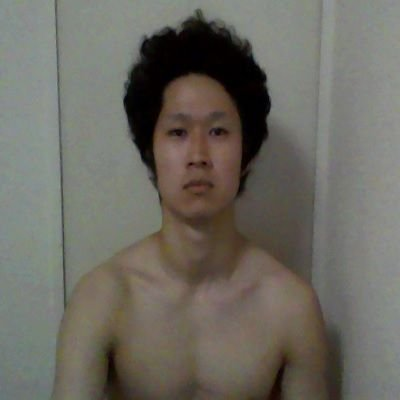
\includegraphics[scale=1]{sutehage.png}
  \caption{入力画像}
  \label{fig:sutehage}
\end{figure}

\begin{figure}[h]
  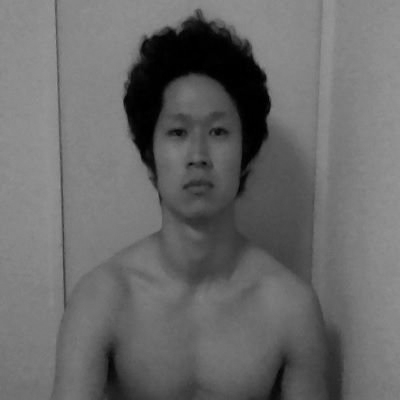
\includegraphics[scale=1]{sutehagegray.png}
  \caption{グレースケール画像}
  \label{fig:sutehage}
  
\end{figure}

\begin{figure}[h]
  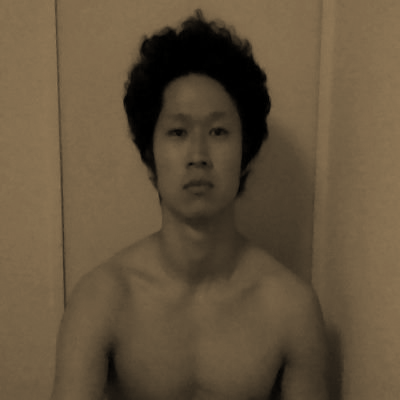
\includegraphics[scale=1]{sutehagesepia.png}
  \caption{セピア}
  \label{fig:sutehage}
  
\end{figure}

\begin{figure}[h]
  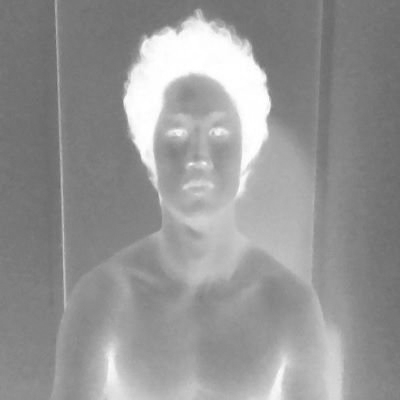
\includegraphics[scale=1]{sutehagenega.png}
  \caption{ネガ}
  \label{fig:sutehage}
  
\end{figure}

\begin{figure}[h]
  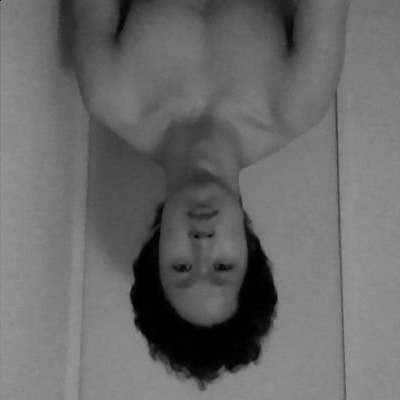
\includegraphics[scale=1]{sutehagereverse.png}
  \caption{上下左右反転}
  \label{fig:sutehage}
  
\end{figure}

\begin{figure}[h]
  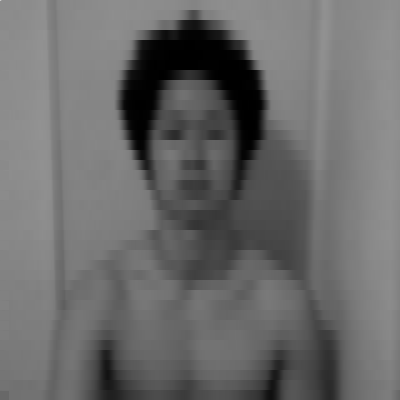
\includegraphics[scale=1]{sutehagemosaic.png}
  \caption{グレースケールモザイク画像}
  \label{fig:sutehage}
  
\end{figure}

\begin{figure}[h]
  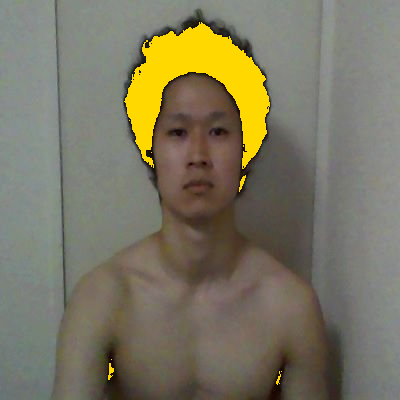
\includegraphics[scale=1]{sutehageb2y.png}
  \caption{サイヤ人}
  \label{fig:sutehage}
  
\end{figure}



\begin{comment}
\section{課題1-2}

\subsection{source}
\lstinputlisting[basicstyle=\ttfamily\footnotesize,frame=single]{a1-2.c}


\subsection{result}
\begin{lstlisting}[basicstyle=\ttfamily\footnotesize,frame=single]
  
\end{lstlisting}
\end{comment}


\end{document}
